% Fig 3: Min-entropy comparison bar chart
\begin{figure}[t]
\centering
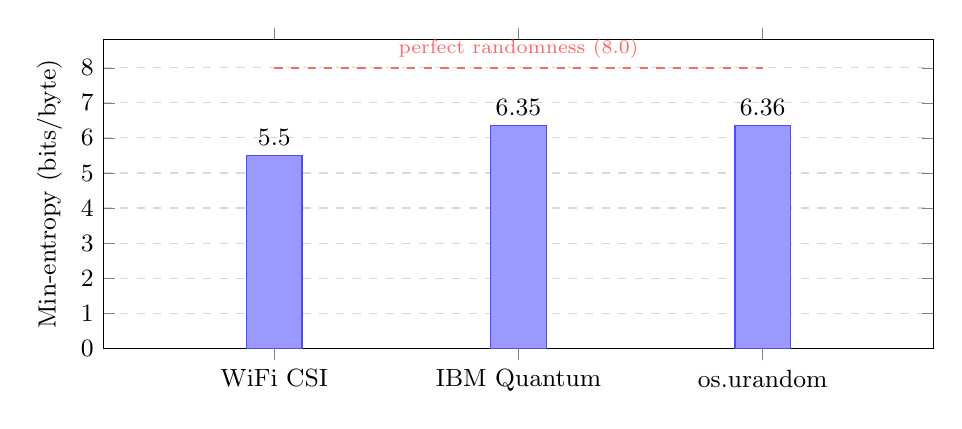
\begin{tikzpicture}
\begin{axis}[
  ybar,
  width=\columnwidth,
  height=5.5cm,
  bar width=20pt,
  ymin=0, ymax=8.8,
  ylabel={Min-entropy (bits/byte)},
  ylabel style={font=\small},
  symbolic x coords={WiFi CSI, IBM Quantum, os.urandom},
  xtick=data,
  xticklabel style={font=\small},
  yticklabel style={font=\small},
  nodes near coords,
  nodes near coords style={font=\small\bfseries, anchor=south},
  enlarge x limits=0.35,
  ymajorgrids=true,
  grid style={dashed, gray!30},
  ytick={0,1,2,3,4,5,6,7,8},
]
\addplot[fill=blue!40, draw=blue!70] coordinates {
  (WiFi CSI, 5.50) (IBM Quantum, 6.35) (os.urandom, 6.36)
};
% Perfect randomness line
\draw[dashed, red!60, thick] (axis cs:WiFi CSI, 8.0) -- (axis cs:os.urandom, 8.0);
\node[font=\scriptsize, text=red!60, anchor=south] at (axis cs:IBM Quantum, 8.0) {perfect randomness (8.0)};
\end{axis}
\end{tikzpicture}
\caption{NIST SP~800-90B final min-entropy assessment (\texttt{ea\_non\_iid}, byte-level, 99\% confidence). WiFi CSI achieves 5.50~bpb (69\% of theoretical maximum), compared to 6.35 for IBM Quantum (ibm\_kingston, 156~qubits) and 6.36 for \texttt{os.urandom}. The CSI result is the first SP~800-90B assessment of WiFi CSI data.}
\label{fig:minentropy-bars}
\end{figure}
